% Preámbulo
\documentclass[letterpaper]{article}
\usepackage[utf8]{inputenc}
\usepackage[spanish]{babel}

\usepackage{enumitem}
\usepackage{titling}

% Símbolos
	\usepackage{amsmath}
	\usepackage{amssymb}
	\usepackage{amsthm}
	\usepackage{amsfonts}
	\usepackage{mathtools}
	\usepackage{bbm}
	\usepackage[thinc]{esdiff}
	\allowdisplaybreaks

% Márgenes
	\usepackage
	[
		margin = 1.2in
	]
	{geometry}

% Imágenes
	\usepackage{float}
	\usepackage{graphicx}
	\graphicspath{{imagenes/}}
	\usepackage{subcaption}

% Macros
	\newcommand{\sumi}[2]{\sum_{i=#1}^{#2}}
	\newcommand{\dint}[2]{\displaystyle\int_{#1}^{#2}}
	\newcommand{\inte}[2]{\int_{#1}^{#2}}
	\newcommand{\dlim}{\displaystyle\lim}
	\newcommand{\limxinf}{\lim_{x\to\infty}}
	\newcommand{\limninf}{\lim_{n\to\infty}}
	\newcommand{\dlimninf}{\displaystyle\lim_{n\to\infty}}
	\newcommand{\limh}{\lim_{h\to0}}
	\newcommand{\ddx}{\dfrac{d}{dx}}
	\newcommand{\txty}{\text{ y }}
	\newcommand{\txto}{\text{ o }}
	\newcommand{\Txty}{\quad\text{y}\quad}
	\newcommand{\Txto}{\quad\text{o}\quad}
	\newcommand{\si}{\text{si}\quad}

	\newcommand{\etiqueta}{\stepcounter{equation}\tag{\theequation}}
	\newcommand{\tq}{:}
	\renewcommand{\o}{\circ}
	% \newcommand*{\QES}{\hfill\ensuremath{\boxplus}}
	% \newcommand*{\qes}{\hfill\ensuremath{\boxminus}}
	% \newcommand*{\qeshere}{\tag*{$\boxminus$}}
	% \newcommand*{\QESHERE}{\tag*{$\boxplus$}}
	\newcommand*{\QES}{\hfill\ensuremath{\blacksquare}}
	\newcommand*{\qes}{\hfill\ensuremath{\square}}
	\newcommand*{\QESHERE}{\tag*{$\blacksquare$}}
	\newcommand*{\qeshere}{\tag*{$\square$}}
	\newcommand*{\QED}{\hfill\ensuremath{\blacksquare}}
	\newcommand*{\QEDHERE}{\tag*{$\blacksquare$}}
	\newcommand*{\qel}{\hfill\ensuremath{\boxdot}}
	\newcommand*{\qelhere}{\tag*{$\boxdot$}}
	\renewcommand*{\qedhere}{\tag*{$\square$}}

	\newcommand{\suc}[1]{\left(#1_n\right)_{n\in\N}}
	\newcommand{\en}[2]{\binom{#1}{#2}}
	\newcommand{\upsum}[2]{U(#1,#2)}
	\newcommand{\lowsum}[2]{L(#1,#2)}
	\newcommand{\abs}[1]{\left| #1 \right| }
	\newcommand{\bars}[1]{\left \| #1 \right \| }
	\newcommand{\pars}[1]{\left( #1 \right) }
	\newcommand{\bracs}[1]{\left[ #1 \right] }
	\newcommand{\floor}[1]{\left \lfloor #1 \right\rfloor }
	\newcommand{\ceil}[1]{\left \lceil #1 \right\rceil }
	\newcommand{\angles}[1]{\left \langle #1 \right\rangle }
	\newcommand{\set}[1]{\left \{ #1 \right\} }
	\newcommand{\norma}[2]{\left\| #1 \right\|_{#2} }


	\newcommand{\N}{\mathbb{N}}
	\newcommand{\Q}{\mathbb{Q}}
	\newcommand{\R}{\mathbb{R}}
	\newcommand{\Z}{\mathbb{Z}}
	\newcommand{\PP}{\mathbb{P}}
	\newcommand{\1}{\mathbbm{1}}
	\newcommand{\eps}{\varepsilon}
	\newcommand{\ttF}{\mathtt{F}}
	\newcommand{\bfF}{\mathbf{F}}

	\newcommand{\To}{\longrightarrow}
	\newcommand{\mTo}{\longmapsto}
	\newcommand{\ssi}{\Longleftrightarrow}
	\newcommand{\sii}{\Leftrightarrow}
	\newcommand{\then}{\Rightarrow}

	\newcommand{\pTFC}{{\itshape 1er TFC\/}}
    \newcommand{\sTFC}{{\itshape 2do TFC\/}}
    
% Datos
    \title{Gráficas y Combinatoria\\Tarea V}
    \author{Rubén Pérez Palacios\\Profesor: Dr. Octavio Arizmendi Echegaray}
    \date{\today}

% DOCUMENTO
\begin{document}
	\maketitle
    
    \section*{Problemas}

    \begin{enumerate}
		
		\item Prueba que todo árbol $T$ tiene al menos $\Delta(T)$ hojas.
		
		Lo demostraremos por inducción sobre el número de vertices $n$.

		\begin{itemize}
			\item \textbf{Caso base:} n = 1
			
			Es cierto puesto que $\Delta(T) = 0$ y el número de hojas es $1$.

			\item \textbf{Hipotesis:}
			
			Todo árbol tiene al menos $T$ tiene al menos $\Delta(T)$ hojas.

			\item \textbf{Paso Inductivo:}
			
			Sea $G$ una árbol con $n+1$ vértices y $u$ un hoja de $G$. Luego entonces $G\setminus u$ es un arbol de $n$ vértices donde a lo más pudimos haber disminuido en $1$ a $\Delta(G)$ y al núemro de hojas, ahora por inducción matemática tenemos que el número de hojas de $G\setminus u$ es al menos $\Delta(T)$ por lo que el único caso que nos genera conflicto es que se de la igualdad, de ser así entonces $G\setminus u$ todos sus nodos excepto $v$ tal que $deg(v) = \Delta(G\setminus u)$ tendrían un grado menor o igual a $2$ de no ser así habría mas hojas que $\Delta(T)$ por lo que si a este grafo le quitamos una hoja $w$ entonces tenemos dos casos cuando $(v,w) \in E(G\setminus u)$ pero de ser así entonces tanto $\Delta(G)$ como el número de hojas disminuirian en $1$, luego si $(v,w) \not\in E(G\setminus u)$ entonces el número de hojas ni $\Delta(G)$ disminuirian. Por lo tanto concluimos que el número de hojas de $G$ es al menos $\Delta(G)$.
		
		\end{itemize}

		\item Para una gráfica con cuello al menos $g  = 2r$ y de grado mínimo mayor que $d$ tiene al menos
		
		\[\sum_{i=0}^{r-1} \pars{d-1}^i\]

		vertices.

		\item Muestre que $K_{3,3}$ no es planar.
		
		Supongamos que $K_{3,3}$ es planar entonces por la formula de Euler tenemos que

		\[V-E+F=2,\]

		donde $V = 6$, $E = 9$, por lo tanto

		\[F = 5.\]

		Ahora veamos de al menos cuantas aristas estan formadas las caras. El número de aristas no puede ser impar ya que el $K_{3,3}$ es bipartito. Entonces el número de aristas por cara al menos es $4$, por lo que el total de aristas que bordean las caras deben ser al menos $4F$, luego al solo poder pertenecer a lo mas $2$ caras cada arista entonces tenemos que $E$ es al menos $2F$ por lo que

		\[E \geq 10,\]

		lo cual cual es una contradicción ya que $E = 9$.

		\item Determine el grado promedio, número de aristas, grado, radio, diametro, cuello y conexidad por aristas del cubo de dimensión $n$.

		\begin{itemize}
			\item \textbf{Grado Promedio:} Se demostrara que todos los vertices tienen el mismo grado digamos el cual es $n$ por inducción sobre $n$.
			Cuando $n = 1$ tendremos una solo arista en el hipercubo por lo que el grado de sus vertices es $1$. Sea $S$ una cadena de $0$ y $1$ de tamaño $n+1$ y sea $T$ la cadena que resulta de quitar el último elemento de $S$ por lo que $T$ es de tamaño $n$, por hipotesis de inducción el número de vertices adyacentes a $T$ son $N$. El número de vertices adyacentes a $S$ son el número de vértices de $T$ mas uno ya que son todas las cadenas que terminan en el mismo elemento que $S$ y que difieren en a lo mas en $1$ en las $n$ posiciones anteriores - de las cuales son la misma cantidad que de vertices de $T$ - y las cadena que es igual en las primeras $n$ posiciones y en la ultima difiere con $S$. por lo tanto concluimos que el grado de todo vertice es $n$ y por lo tanto también su promedio.
			\item \textbf{Aristas:} Puesto que la cantidad de vertices es $2^n$, al ser el grado de cada vertice $n$ entonces este genera $n$ pero al ser cada arista compuesta por dos vertices entonces concluimos que la cantidad de aristas es
			
			\[\frac{2^{n}n}{2} = 2^{n-1}n.\]
			\item \textbf{Radio y Diametro:} Veamos que la distancia entre los vertices cuyas cadenas $S$ y $T$ difieren en todos las posiciones es la excentrecidad de ambos y por lo tanto $n$, esto puesto que de no ser así entonces existe un $R$ tal que su distancia a $S$ es mayor que la de $S$ a $T$ pero $R$ difiere en menos de $n$ posiciones digamos $k$ por lo que si seguimos el camino $S_0\sim S_1 \sim \cdots \sim S_{k-1} \sim S_{k}$ donde $S_0 = S, S_k = R$ y $S_{i+1}$ es igual a la cadena $S_i$ excepto en primera posición donde difieren $S_i$ y $R$, donde en esa posición la cedan $S_{i+1}$ es igua a $R$, luego entonces este al ser un camino de tamaño $k <= n$ es una contradicción que $R$ es un punto a mayor distancia que $T$. Tomando el mismo camino anterior tenemos que la $dist(S,T) \leq n$ pero si fuese menor que $n$ entonces tendriamos dos nodos conexos que difieren en mas de una posición por lo que la excentricidad de $S$ y $T$ es $n$. Por lo tanto concluimos que tanto el radio como el diametro son iguales a $n$.
			\item \textbf{Cuello:} Una cara consta de $4$ aristas, vertices puesto que no puede ser $3$ ya que de ser así entonces dos vertices cuyas secuencias diferirian en $2$ posiciones por lo que no pueden estar conectadas; y es de $4$ ya que consideremos los vertices adyacentes que al menos tiene una cara $F$ digamos $A$, $B$ y $C$ tales que $(A,B),(B,C)$ son aristas, luego sabemos que la cadena que representa $A$ difiere en una posición $i$ a la de $B$ y así mismo la cadena que representa a $B$ difiere en una posición $j$ a la de $C$; $i$ y $j$ no pueden ser iguales ya que der asi entonces $A = C$, luego entonces tenemos que $A$ y $C$ difieren en las posiciones $i$ y $j$ por lo que estos dos tienen dos vecinos en común donde uno de ellos es $B$ y el otro es $D$ y por lo tanto se tiene un ciclo de tamaño $4$ el cual es la cara $F$. Puesto que cada ciclo es de al menos $4$ vertices entonces el cuello es $4$.
			\item \textbf{Conexo:} Sean $U$ y $V$ vertices en el hipercubo y $S$ y $T$ las cadenas que los representan respectivamente. Demostremos que siempre hay un camino entre $U$ y $V$, para ello lo divideremos en dos casos cuando $S$ y $T$ coinciden o no en su úlitma posición. Para lo primero lo haremos a través de inducción. Para $n = 1$ puesto que solo se tienen $2$ vertices y una arista entre ellos se cumple que es conexo. Consideremos el hipercubo de dimensión $n+1$ y $U,V,S,T$ como se describieron anteriormente, y sea $S',T'$ cadenas de tamaño $n$ tales que cada posición de $S'$ coincide con la de $S$ y cada posición de $T'$ coincide con la de $T$, entonces por hipotesis de inducción existe un camino $R_1'\sim R_2' \sim \cdots \sim R_{k-1}' \sim R_k'$ tal que $R_1' = S'$, $R_k' = T'$, entonces sean $R_1,\cdots, R_k$ tales que cada entrada de $R_i'$ coincide con la de $R_i$ y la ultima posición de $R_i$ es la misma que la de $S$ la cual también es la de $T$, entonces tenemos que $R_1 \sim R_2 \sim \cdots \sim R_{k-1} \sim R_k$ es un camino entre $S$ y $T$. Ahora cuando $S$ y $T$ difieren en una posición entonces tomamos $R$ tal que $R$ coincide en la primeras $n$ posiciones con $T$ y en la ultima posición es igual a $S$ entonces sabemos que $T$ y $R$ estan conectados y por lo anterior $R$ y $S$ están conectados por lo tanto $S$ y $T$ también lo estan.
		\end{itemize}

		\item Determine el polinomio cromático de la siguiente gráfica
		
		\begin{figure}[H]
			\centering
			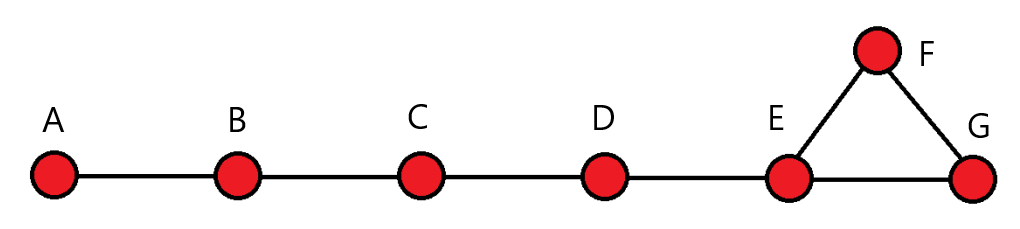
\includegraphics[scale = 0.5]{Images/graph.png}
		\end{figure}

		Nos refiremos a este gráfica por $G$. Por la recurción del polinomio Característico de un gráfica tenemos que

		\[P(G,k) = P(G-ef,k) - P(G/ef,k).\]

		Al ser $G-ef$ un árbol con $7$ nodos tenemos que su polinomio caráctieristico es

		\[P(G-ef,k) = k(k-1)^{6}.\]

		Asi mismo al ser $G/ef$ un árbol con $6$ nodos tenemos que su polinomio caráctieristico es

		\[P(G/ef,k) = k(k-1)^{5}.\]

		Por lo tanto concluimos que

		\[P(G,k) = k(k-1)^6 - k(k-1)^5 = k(k-1)^5(k-1-1) = k(k-1)^5(k-2).\]

    \end{enumerate}

	\end{document}
